\chapter{Dust Attack}
Il dust attack è una nota tecnica, presente nel mondo delle criptovalute, il cui obiettivo è la 
de-anonimizzazione del proprietario di un wallet. L'obiettivo dell'attaccante è di collegare address diversi tra loro, ovvero riuscire a capire quali address appartengano ad uno stesso wallet.\\

\section{Strategia di attacco}
La strategia usata dagli attaccanti è quella di inviare a diversi address piccoli importi dust.\\
In Bitcoin, il termine dust si riferisce agli importi inferiori alla fee minima richiesta per spenderli in una transazione. Come specificato in \cite{BtcDev}, un
importo è considerato dust se è inferiore alla soglia di 546 satoshi.\\
Per effettuare il dust attack quindi è necessario avere a disposizione una certa quantità di bitcoin da poter dividere in centinaia, o migliaia, di output dust.
L'attaccante invia questi piccoli importi nella speranza che vengano spesi successivamente in una nuova transazione insieme ad altri address, poiché, come spiegato nel capitolo precedente, è raro che gli address di input appartengano a più utenti, si presume che tutti gli address appartengano a una sola persona; quindi sono collegati tra loro.
\begin{figure}[h!]
    \centering
    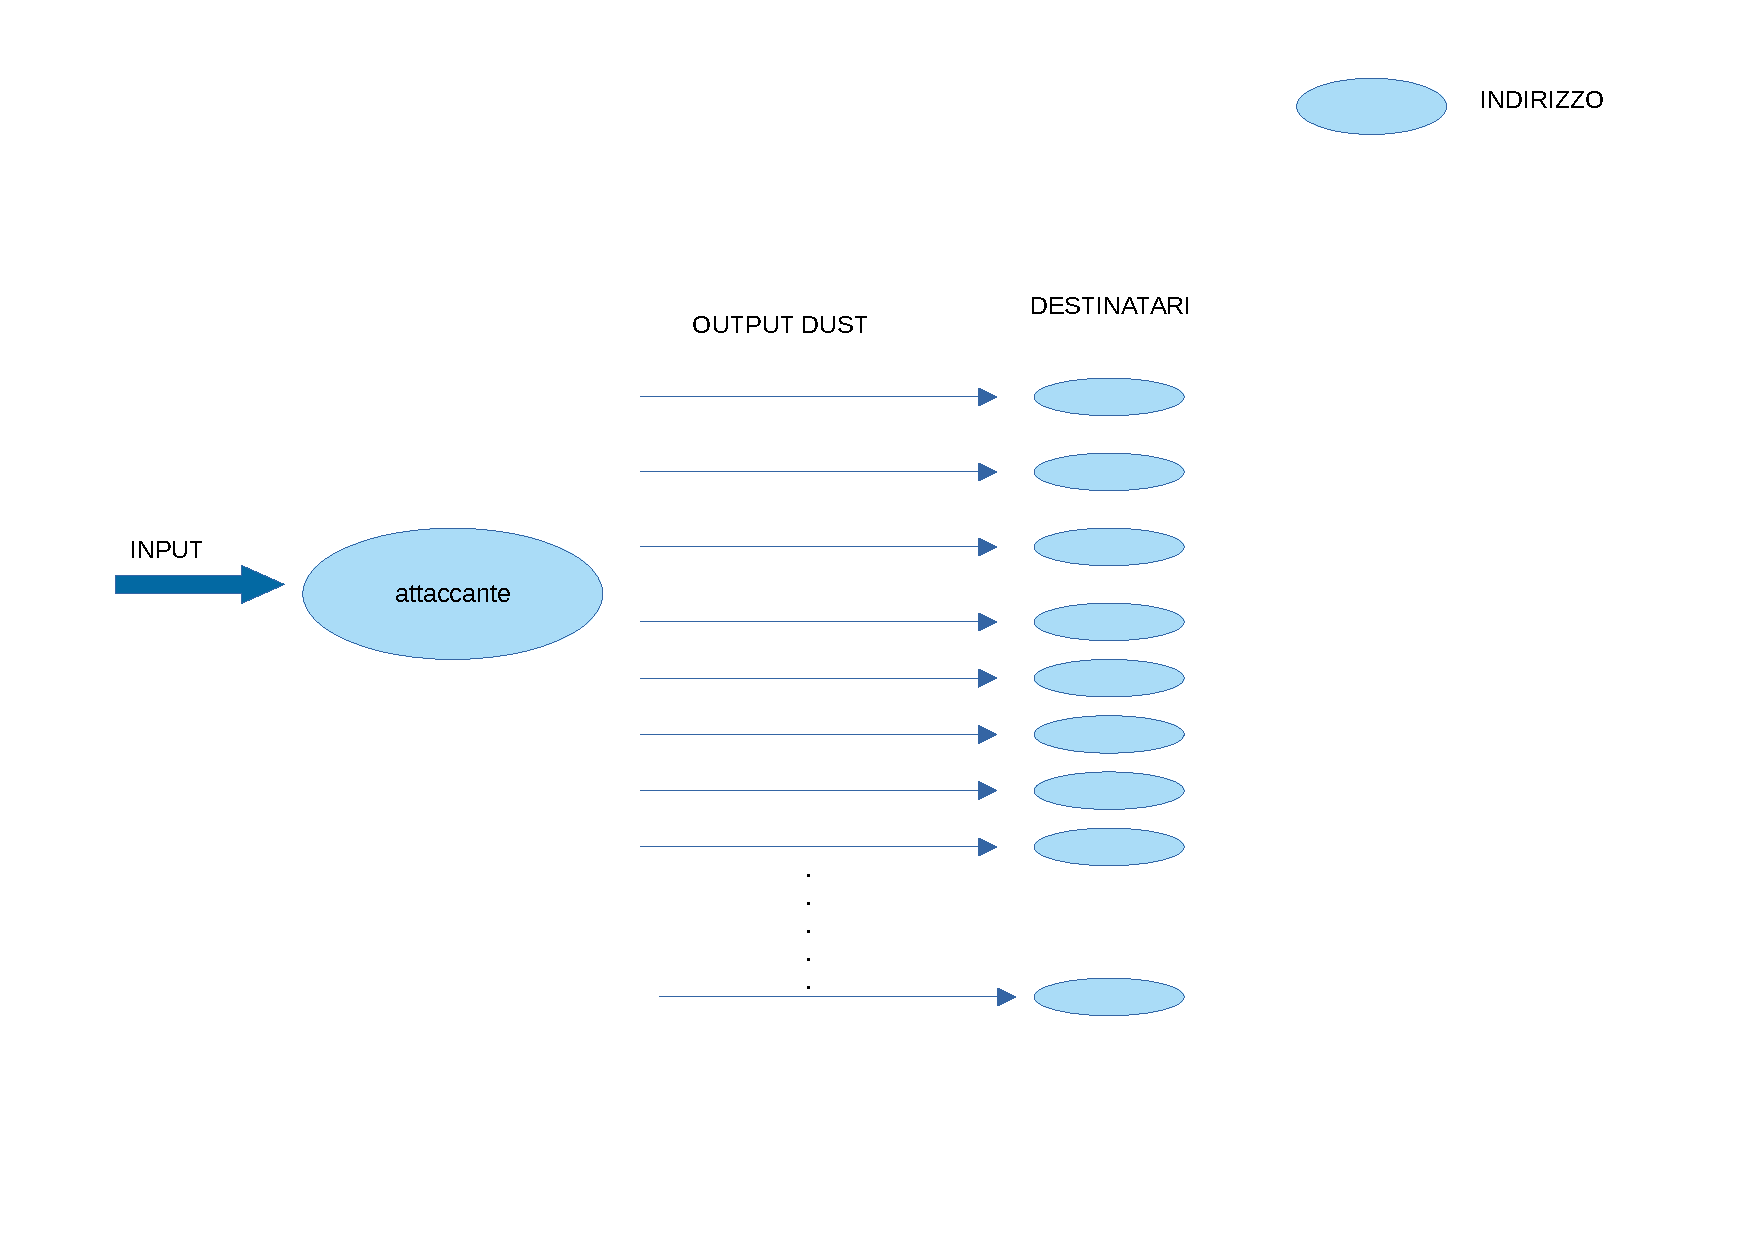
\includegraphics[scale=0.5]{Images/dust_attack.pdf}
    \caption{Schema Dust Attack}
    \label{fig:Dust_attack}
\end{figure}
\FloatBarrier
Una volta effettuato l'attacco possono esserci tre possibili esiti: 
    \begin{enumerate}
        \item attacco di successo;
        \item attacco fallito;
        \item dust bruciato.
    \end{enumerate}
Nel primo caso la vittima genera una transazione in cui spende l'importo dust ricevuto insieme ad almeno un altro dei suoi address. L'attaccante può quindi collegarli e capire che appartengono alla stessa persona.\\\\
\begin{figure}[h!]
    \centering
    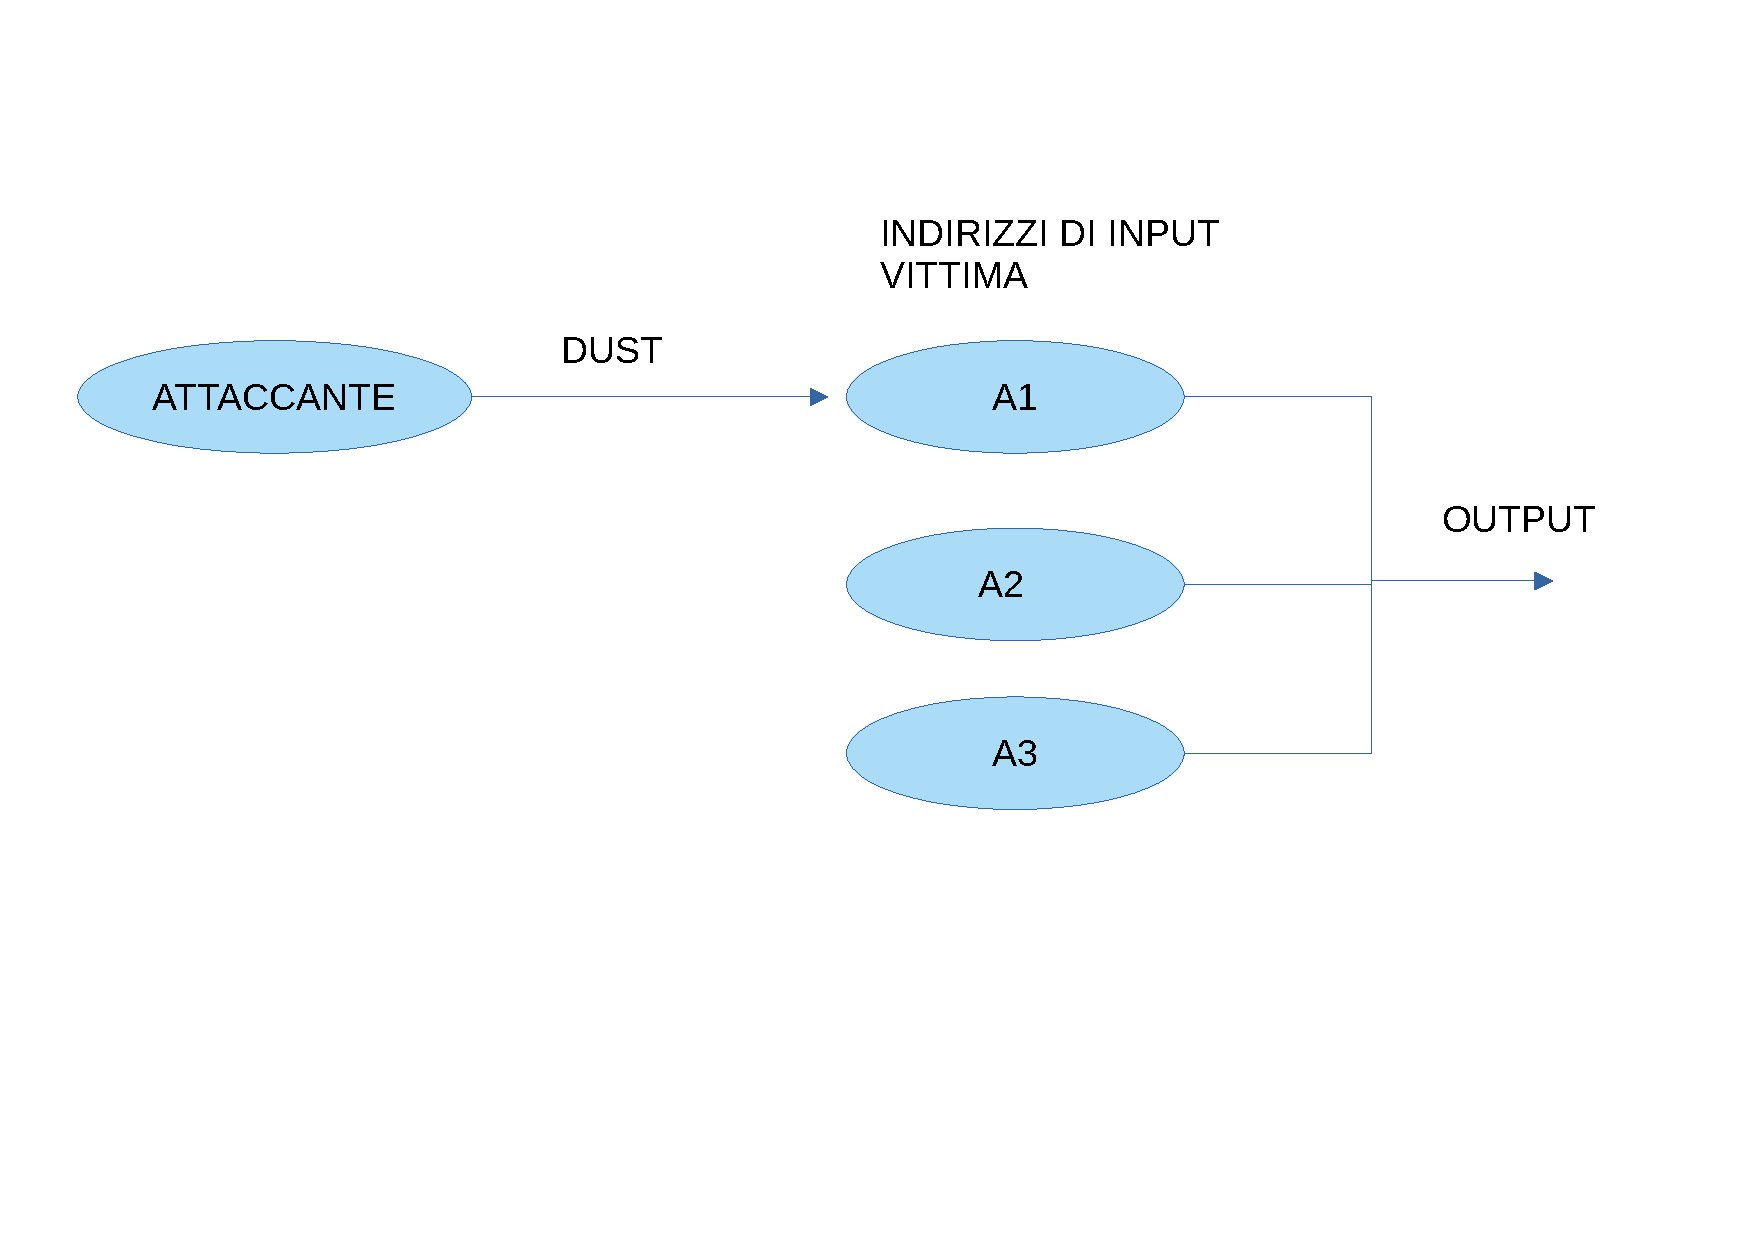
\includegraphics[scale=0.3]{Images/successo.pdf}
    \caption{Schema Attacco di Successo}
    \label{fig:success}
\end{figure}
\FloatBarrier
Nel secondo caso invece l'importo è stato speso in una transazione dove sono presenti più input ma tutti legati allo stesso address. In questa situazione l'attaccante non collega address diversi e quindi fallisce nel tentativo di de-anonimizzazione. 
\begin{figure}[h!]
    \centering
    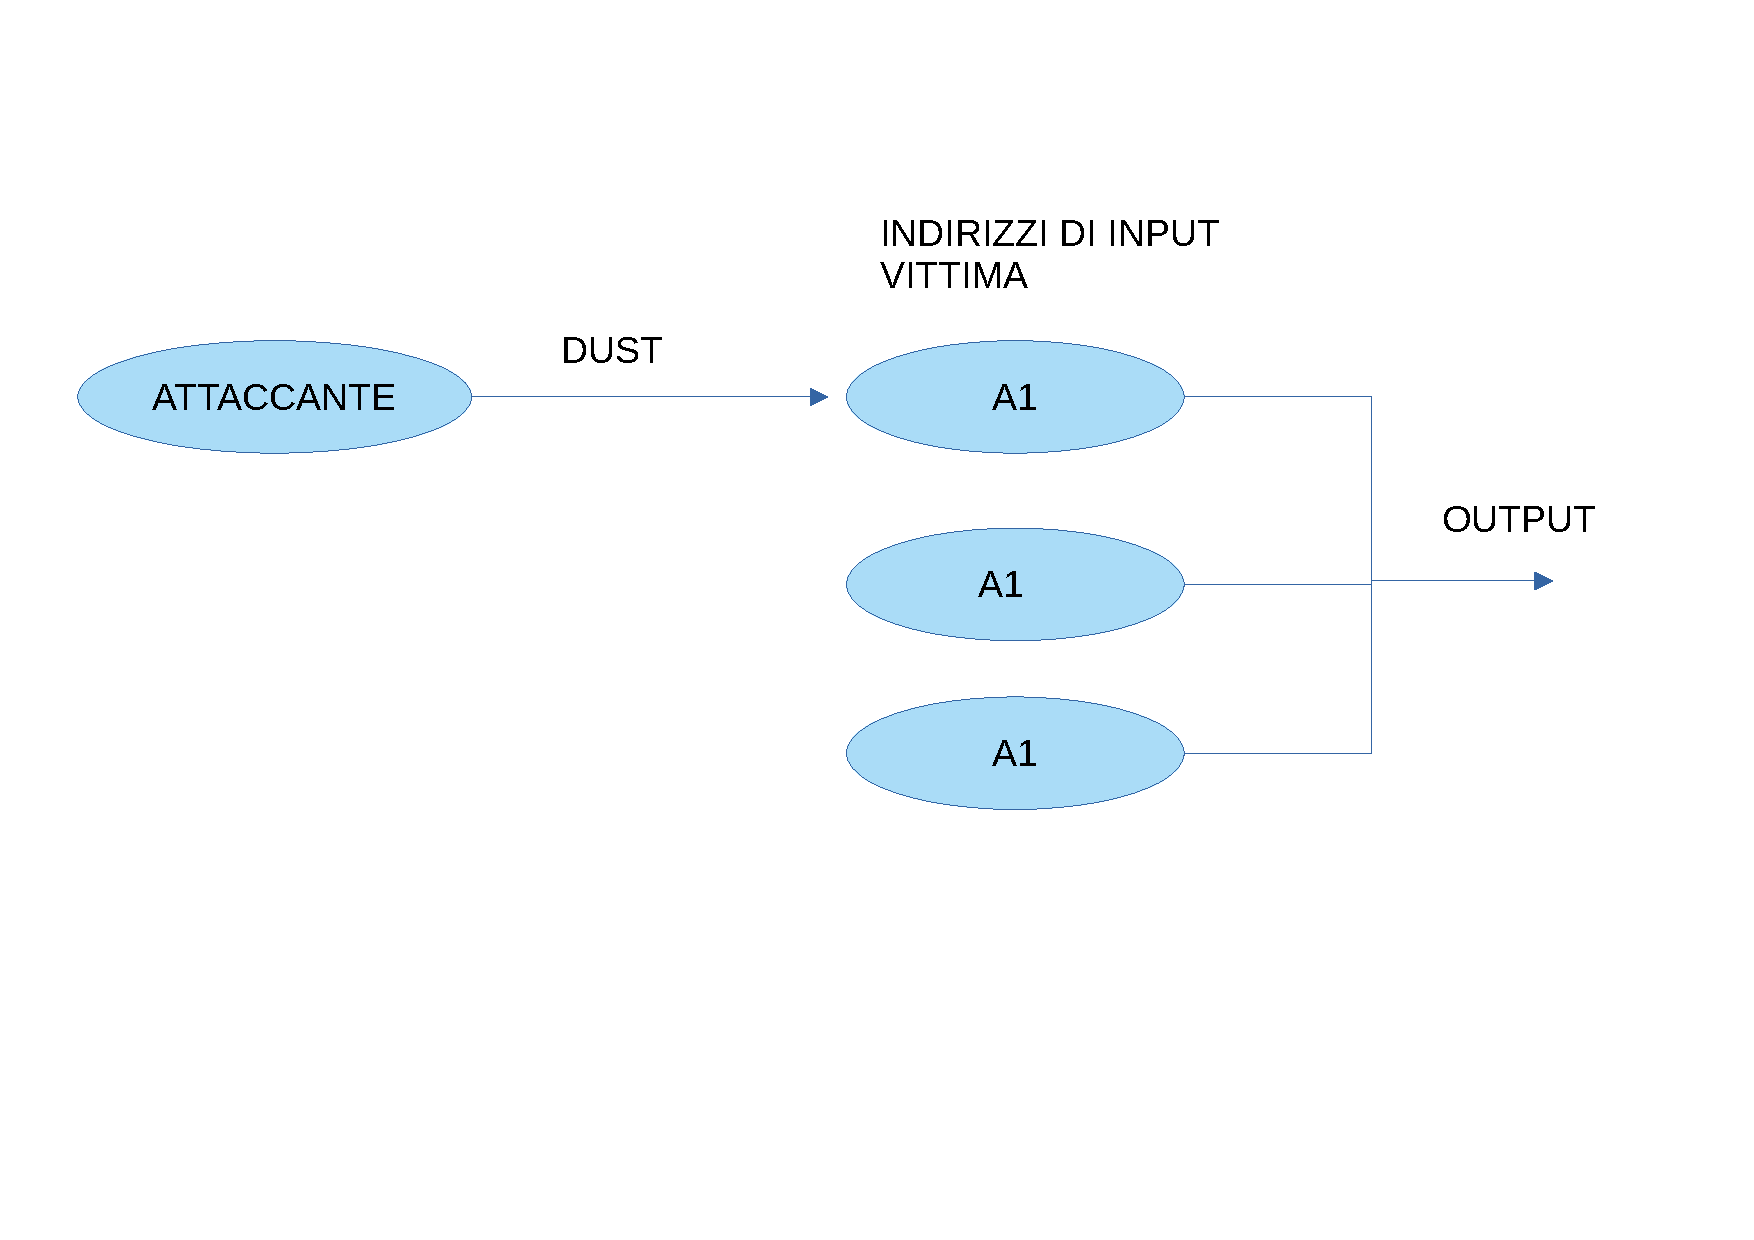
\includegraphics[scale=0.35]{Images/fallimento.pdf}
    \caption{Schema Attacco Fallito}
    \label{fig:fallito}
\end{figure}
\FloatBarrier
Il \textit{dust attack} quindi risulta più efficace soprattutto contro gli address che hanno un bilancio complessivo pari a zero proprio perché obbliga la vittima a spendere la cifra ottenuta con altri suoi address diversi.\\\\
Terzo e ultimo caso semplicemente la vittima non spende il dust ricevuto troncando l'attacco sul nascere.\\\\
Bisogna specificare che il dust attack non permette di rubare fondi di altri utenti né permette di scoprire le informazioni personali, per esempio nome e cognome, della vittima ma permette di ricavare un'importante informazione che può essere usata in seguito per effettuare attacchi più pericolosi.
\section{Conseguenze}
Come detto prima questa tipo di de-anonimizzazione di per sé non costituisce un problema. Può diventarlo se viene usata come mezzo per altri tipi di attacchi. In generale il Dust Attack non per forza è legato a phishing o estorsioni ma potrebbe essere usato dalle autorità per tenere traccia degli utenti ed eventualmente rilevare attività illegali. Infatti una volta otteuto un cluster di address riesco a tracciare l'attività di un singolo utente e non più di un singolo address. Le autorità potrebbero notare che certi utenti interagiscono con address legati a mercati neri, e quindi indagare ulteriormente per scoprire l'identità di queste persone. Uno dei punti fondamentali è legare informazioni personali, come e-mail, nome ed altro, a address Bitcoin. In molti casi sono gli utenti stessi che pubblicano sui forum i loro address, in altre situazioni invece è possibile sfruttare gli exchange come Coinbase.\\\\Gli exchange sono servizi che permettono lo scambio tra criptovalute e valute tradizionali basandosi sul valore di mercato della criptovaluta. In exchange come Coinbase è necessario creare un account fornendo informazioni personali come nome, cognome, email ed altro e, una volta registrati, viene creato un wallet associato a quel particolare account. Siccome gli exchange sono esposti ad attacchi hacker molti utenti trasferiscono i loro bitcoin su address appartenenti a software wallet, per esempio Wasabi Wallet.\\\\
Una volta che un utente effettua un deposito dal wallet, vittima di Dust Attack, ad un account exchange ecco che l'attaccante collega gli address al proprietario. Una volta ottenuta l'identità del proprietario l'attaccante può eseguire elaborati attacchi di phishing oppure può estorcergli il denaro minacciandolo di rivelare a tutti l'informazione ottenuta.\\ Il Dust Attack però non risulta particolarmente difficile da contrastare, nel paragrafo successivo spiegherò due metodi per difendersi da questo tipo di attacco.
\section{Contromisure}
Due metodi per contrastare il dust attack sono:
    \begin{enumerate}
        \item non spendere l'importo dust ricevuto; 
        \item utlizzare servizi di "dust collecting". 
    \end{enumerate}
La prima soluzione, semplice ed efficace, permette di troncare l'attacco sul nascere. Infatti se il dust non viene speso l'attaccante non potrà mai collegare gli address. 
Questo metodo può esserre effettuato in diversi software wallet; per esempio Samurai Wallet\footnote{fonte:\url{https://twitter.com/samouraiwallet/status/1055345822076936192?lang=en}}, nel 2018, consigliò ai suoi utenti, possibili vittime di \textit{dust attack},  di contrassegnare come "do not spend" le UTXO in questione.\\\\
La seconda soluzione riguarda i servizi di "dust collecting", per esempio Dust-B-Gone\cite{Dbg}.
L'obiettivo di questo meccanismo è di impedire la de-anonimizzazione tramite la generazione di una singola transazione dove gli input dust provengono da utenti diversi. L'importo complessivo viene trasformato in fee per i miners. \\Siccome gli address di input appartengono a persone differenti, l'attaccante fallisce nel tentativo di de-anonimizzazione.